\subsection{Comparación de algoritmos}

En esta sección, comparamos varios algoritmos con respecto a nuestras métricas de interés: Accuracy, Precision, Recall y F1 Score (R2). Los algoritmos considerados se dividen en:

\subsubsection*{Clasificación:}

\begin{itemize}
    \item DecisionTreeClassifier
    \item LogisticRegression
    \item RandomForestClassifier
    \item XGBClassifier
\end{itemize}

Para estos modelos, se utilizará la variable objetivo \say{aprobado}, la técnica \say{Stratified K-Fold Cross-Validation}, ajustaremos el mejor modelo en los datos de entrenamiento y realizaremos predicciones utilizando el mejor modelo.

La mejor configuración para los modelos de clasificación se muestra en la Figura \ref{fig:config_clasifiacion}:

\begin{figure}[H]
    \centering
    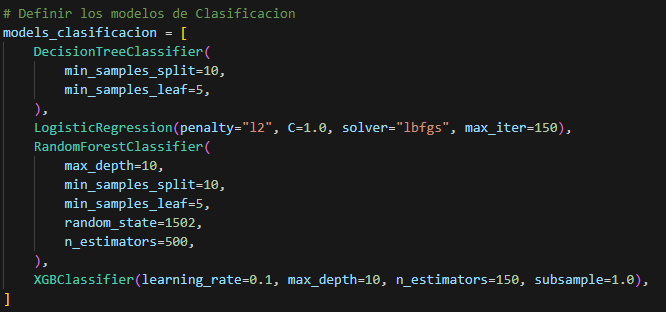
\includegraphics[width=6.06111in,height=2.68611in]{img/compara_algoritmos/configModelsClasificacion.png}
    \caption{Configuración de los modelos de clasificación}
    \label{fig:config_clasifiacion}
\end{figure}

Los resultados obtenidos se presentan en la Figura \ref{fig:metricas_clasificacion}:

\begin{figure}[H]
    \centering
    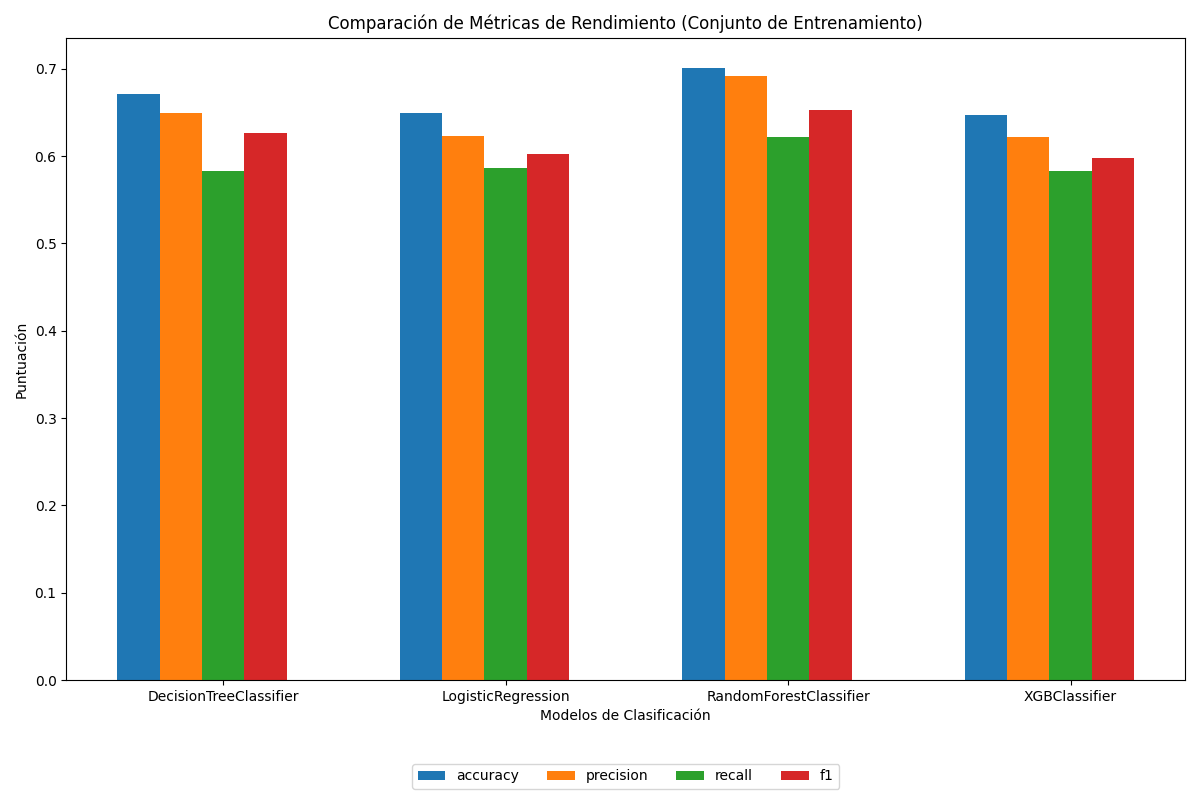
\includegraphics[width=7.06111in,height=4.68611in]{img/compara_algoritmos/metricasEntreModelosClasificacion.png}
    \caption{Métricas entre modelos de clasificación}
    \label{fig:metricas_clasificacion}
\end{figure}

Se observa que el modelo RandomForestClassifier es el mejor modelo, con un F1 Score del 62.08\%, un recall del 58.67\%, una precisión del 66.54\% y una exactitud del 68.11\%, en comparación con los otros modelos evaluados.

\subsubsection*{Regresión:}

\begin{itemize}
    \item LinearRegression
    \item DecisionTreeRegressor
    \item KNeighborsRegressor
\end{itemize}

Para estos modelos, se utilizará la variable objetivo \say{sol1}, la técnica \say{K-Fold Cross-Validation}, ajustaremos el mejor modelo en los datos de entrenamiento y realizaremos predicciones utilizando el mejor modelo.

La mejor configuración para los modelos de regresión se muestra en la Figura \ref{fig:config_regresion}:

\begin{figure}[H]
    \centering
    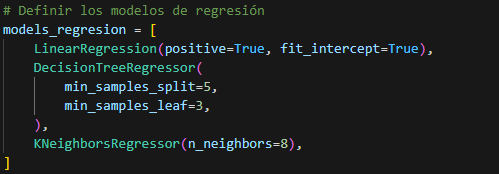
\includegraphics[width=5.06111in,height=1.68611in]{img/compara_algoritmos/configModelsRegresion.png}
    \caption{Configuración de los modelos de regresión}
    \label{fig:config_regresion}
\end{figure}

Los resultados obtenidos se presentan en la Figura \ref{fig:metricas_regresion}:

\begin{figure}[H]
    \centering
    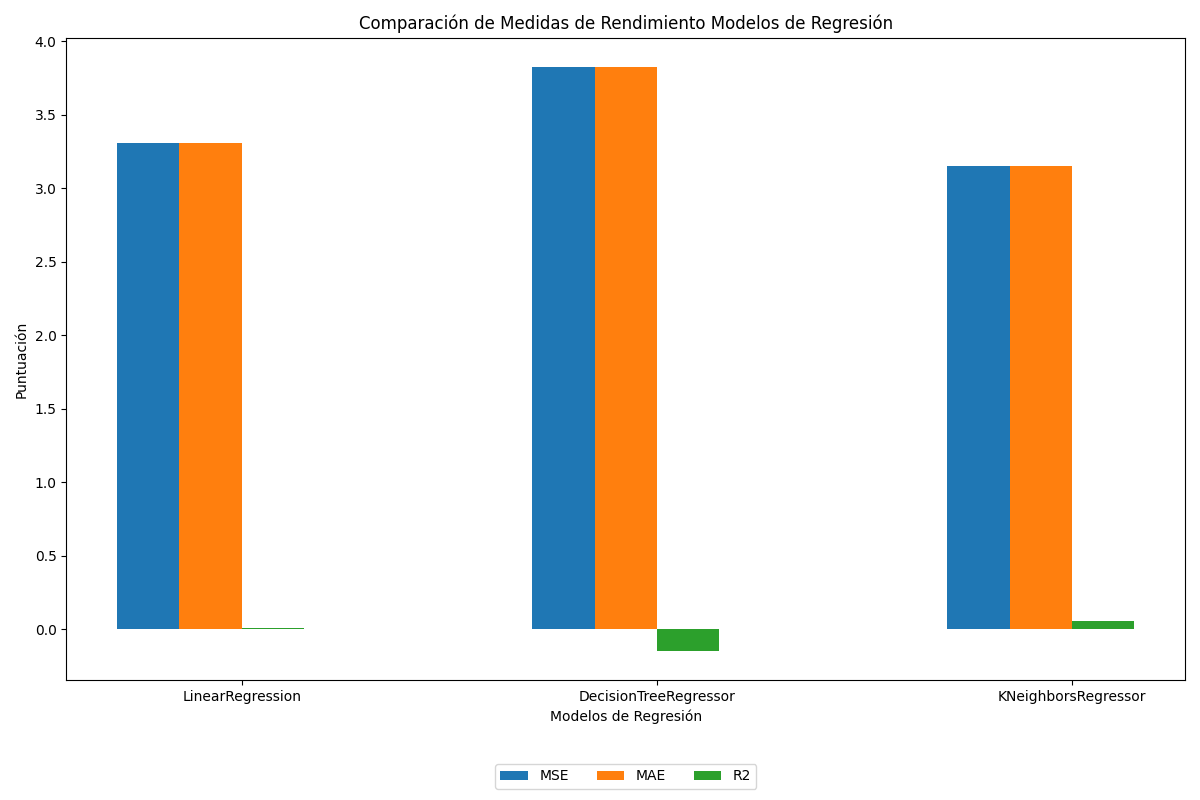
\includegraphics[width=7.06111in,height=4.68611in]{img/compara_algoritmos/metricasEntreModelosRegresion.png}
    \caption{Métricas entre modelos de regresión}
    \label{fig:metricas_regresion}
\end{figure}

Se observa que el modelo LinearRegression es el mejor modelo de regresión, con un MSE del 2.77\% y un MAE del 2.77\%, valores inferiores a los de los otros modelos evaluados. Además, el modelo LinearRegression presenta un R2 más cercano a 1, con un aumento del 0.16\% en comparación con los demás modelos.

En conclusión, se realizó una comparación exhaustiva de diferentes algoritmos de modelos predictivos para determinar cuál es el más adecuado en términos de origen de datos. Después de analizar y comparar varios algoritmos, se llegó a la conclusión de que el modelo RandomForestClassifier se destaca como el enfoque más efectivo para el origen de datos en cuestión, mientras que el modelo LinearRegression es el más adecuado para análisis de regresión.